% Исходный LaTeX-код (c) Пётр Калинин, 2014-
% Код распространяется по лицензии GNU GPL (!)

\documentclass[a4paper,10pt]{problems}
\usepackage{framed}
\usepackage{verbatim}
\let\eps\varepsilon


\begin{document}

\begin{flushright}
Автор: Пётр Калинин, основной текст: 2014\\
Этот документ можно распространять по лицензии\\
Creative Commons Attribution-ShareAlike 3.0 Unported (CC BY-SA 3.0)\\
Последнюю версию, а также исходный код для системы \LaTeX\\
можно скачать с \verb`https://github.com/petr-kalinin/progtexts`\\
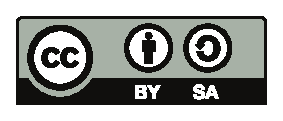
\includegraphics[width=2cm]{by-sa-corr.eps}
\end{flushright}

\Header{Двоичный поиск}

Двоичный поиск, он же бинарный поиск, он же алгоритм деления пополам или дихотимия "--- это целая серия алгоритмов, объединенных одной идеей. 
Мы их последовательно рассмотрим.

\header{Вещественный двоичный поиск}

\lheader{Прочность нити на разрыв}
Для начала рассмотрим следующую задачу "--- не совсем по программированию. Пусть у нас есть, например, нитка. 
Мы можем подвешивать к этой нитке различные грузы, при этом если мы подвесим слишком большой груз, то нитка порвется. 
Соответственно, есть некоторый пороговая масса груза $m_0$ такая, что от любой б\'{о}льшой массы нитка рвется, а от любой меньше "--- нет.
Поставим задачу определить эту пороговую массу.

(Может возникнуть вопрос: а что происходит, если масса точно равна $m_0$? 
Будем считать, что происходит что"=то конкретное, что имеет место только один из следующих вариантов: либо при $m_0$ нитка всегда рвется, либо всегда нет.
На самом деле, это нам совершенно несущественно, как будет видно ниже.)

Будем считать, что запасы нитки у нас достаточно велики "--- ее хватит на проведение большого количества экспериментов.
Будем также считать, что нитка абсолютно невесома (не рвется под своей тяжестью) и однородна, 
т.е. для любого ее куска пороговая масса одна и та же "--- все-таки у нас олимпиады по программированию, а не по физике%
\footnote{Реальные нитки неоднородны и $m_0$ зависит от куска. 
См. \textit{Всероссийские олимпиады по физике, 1992-2001} под ред. С.~М. Козела, В.~П. Слободянина, часть 2, задача 10.17.}%
.
Также будем считать, что нас доступны грузы абсолютно любой (неотрицательной, конечно) массы, с бесконечной точностью 
(т.е. что мы, например, можем сделать груз массы ровно $20\pi+137,035999074$ грамм.

Итак, постараемся определить $m_0$ за минимальное число экспериментов. 
Точнее, конечно, \textit{абсолютно точно} определить $m_0$ у нас не получится, т.к. для этого надо определить бесконечное число десятичных знаков, 
которые могут быть в записи $m_0$. 
Поэтому выберем маленькое число $\eps$ и постараемся найти $m_0$ с точностью $\eps$, 
т.е. найти такие $l$ и $r$, что $l\leq m_0\leq r$, но $r-l\leq \eps$.

Алгоритм достаточно прост. Мы знаем, что если к нити не подвешивать груз (т.е. подвесить груз массы $0$), то она не порвется. 
С другой стороны, будем считать, что мы знаем такую массу $M$, при которой нить точно порвется 
(например, если это обычная швейная нить, то вряд ли она выдержит груз массой 1 тонну).
Соответственно, обозначим эти две величины как $l$ и $r$ и далее будем их корректировать. 
А именно, на каждом шагу алгоритма возьмам среднее арифметическое масс $l$ и $r$ и поставим эксперимент: порвется нитка от такой массы или нет? 
Если порвется, то корректируем границу $r$, иначе $l$:
\begin{codesampleo}\begin{verbatim}
l:=0;
r:=m_big;  // та самая масса M, при которой нить точно рвется
while r-l>eps do begin    // eps --- требуемая точностью
    m:=(r+l)/2;
    if (нить рвется от массы m) then
        r:=m
    else l:=m;
end;
\end{verbatim}
\end{codesampleo}

В результате у нас \textit{всегда} при выполнении алгоритма будет так, что от массы $r$ нить рвется, а от массы $l$ "--- нет. 
В итоге мы и найдем такие $l$ и $r$, что $r-l\leq eps$, и $l\leq m_0\leq r$.

Вернемся к вопросу о том, что происходит с ниткой при массе, точно равной $m_0$, а именно поймем, почему ответ на этот вопрос нам не важен.
Действительно, во"=первых, крайне маловероятно, что в некоторый момент выполнения алгоритма у нас $m$ будет точно равно $m_0$.
Мы ведь проверяем конечное число значений, а $m_0$ может быть любым вещественным числом "--- чтобы мы попали точно в $m_0$,
нам должно очень крупно повезти (строго говоря, вероятность этого "--- например, с учетом случайности отношения $M/m_0$ "--- точно равна нулю).
Но во"=вторых, пусть даже на очередной итерации у нас получилось $m=m_0$, и пусть нитка порвалась. 
Тогда у нас будет $r=m_0$, и при всех дальнейших экспериментах нитка рваться не будет, т.к. везде далее будет $m<m_0$,
в итоге получим $r=m_0$ и $l\approx m_0-\eps$ "--- все равно $m_0$ мы с нужной точностью нашли. 
Совершенно аналогично, если бы при $m=m_0$ нитка не порвалась бы, то мы получили бы $l=m_0$ и $r\approx m_0+\eps$ 
"--- в пределах заданной точности решение то же самое.

Какова сложность алгоритма? Сложность, конечно, будет измерять в количестве экспериментов.
Изначально $r-l=M$, в конце $r-l\approx \eps$, каждый раз $r-l$ уменьшается в два раза,
поэтому общее количество итераций будет примерно $\log_2 (M/eps)$. 
Это не очень много; например, если $M=1e20$, а $eps=1e-20$, то $\log_2 (M/eps)\approx 133$.

\lheader{Общая идея} 
Итак, общая идея уже достаточно понятна. 
Пусть у нас есть некоторый критерий, определяющий, что некоторые вещественные числа являются в каком"=то смысле <<хорошими>>, а некоторые "--- <<плохими>>,
причем все хорошие идут до всех плохих. 
Нам надо определить пороговое значение, где хорошие числа становятся плохими.

Мы поступаем очень просто: берем некоторые два числа, одно из которых ($l_0$) гарантированно является хорошим, а другое ($r_0$) "--- плохим,
и далее много раз повторяем следующую операцию: вычисляем среднее арифметическое $m$ этих двух чисел и смотрим: хорошее оно или плохое.
Если хорошее, то мы можем присвоить $l:=m$, иначе $r:=m$. 
В итоге у нас постоянно $l$ будет хорошим, а $r$ плохим, а на каждом шагу разность $r-l$ будет уменьшаться в два раза 
"--- за примерно $\log_2(M/\eps)$ итераций (где $M$ "--- начальное значение разности $r-l$) мы достигнем точности $\eps$.

Общий алгоритм выглядит почти так же, как и приведенный выше:
\begin{codesampleo}\begin{verbatim}
l:=l0;
r:=r0;
while r-l>eps do begin    
    m:=(r+l)/2;
    if good(m) then
        l:=m
    else r:=m;
end;
\end{verbatim}
\end{codesampleo}

Здесь \verb`good(x)` "--- функция, возвращающая \verb`true`, если $x$ "--- хорошее число, и \verb`false` "--- если плохое. 
Вообще, всегда, когда пишите деление пополам, выносите проверку <<хорошести>> числа в отдельную функцию, чтобы не загромождать основной цикл.
(Исключение см. в следующем разделе.)

Как и в примере выше, нам совершенно не важно, является ли порогое число <<хорошим>> или нет.

\lheader{Поиск корня функции}
Существенный частный случай вещественного двоичного поиска (да и вообще многие вещественные двоичные поиски можно объявить частным случаем этого)
"--- это поиск корня монотонной непрерывной функции.
Итак, пусть у нас есть функция $f(x)$, которая монотонно строго возрастает (по крайней мере на интересующем нас отрезке) 
и непрерывна (т.е. не имеет скачков) там же.
И пусть у нас есть такие два числа $l$ и $r$, что $f(l)\leq0$, а $f(r)\geq0$.

Есть соответствующая теорема математического анализа, что в таком случае на отрезке $[l,r]$ у функции есть ноль,
т.е. такое значение $x_0$, что $f(x_0)=0$, причем такое значение $x_0$ единственно. 
Его легко найти двоичным поиском: просто объявляем все такие $x$, что $f(x)<0$, <<хорошими>>,
а все такие $x$, что $f(x)>0$, "--- <<плохими>>. 
(Как и раньше, нам не важно, каким определить собственно то единственное $x_0$, для которого $f(x_0)=0$.)
И легко пишем алгоритм:
\begin{codesampleo}\begin{verbatim}
while r-l>eps do begin    
    m:=(r+l)/2;
    if f(m)<0 then   // можно и <=
        l:=m
    else r:=m;
end;
\end{verbatim}
\end{codesampleo}

Здесь в условии if'а стоит сравнение $f(m)<0$. 
Это "--- то самое исключение, про которое я писал в предыдущем разделе: если вы ищете корень функции, то можно в поиске в if'е написать
сравнение функции с нулем. Но само вычисление $f(m)$ все равно вынесите в отдельную функцию.

Аналогично можно искать и корень уравнения $f(x)=c$, если вы знаете, что $f(l)\leq c$, а $f(r)\geq c$.

\lheader{А если функция не монотонна или не непрерывна?}
Если функция строго возрастает, но разрывна, то есть риск, что у нее нет корня: что в некоторый момент она делает скачок сразу от отрицательного
значения до положительного (т.е. например $f(x)<0$ при $x\leq x_0$, но $f(x)>0$ при $x>x_0$). 
Но тогда наш алгоритм тоже срабатывает вполне разумно: $l$ и $r$ в итоге будут ограничивать $\eps$"=окрестность этого скачка.

Если функция монотонна, но убывает, а не возрастает, то решение тоже понятно: надо просто изменить знак проверки в \verb`if`, ну или
поменять местами присваивания $l$ и $r$. 

Если заранее неизвестно, возрастает функция или убывает (но известно, что она монотонна), то, конечно, надо ориентироваться на знаки $f(l)$ и $f(r)$.
Можно заранее запомнить знак $f(l)$, но можно написать проще: просто в условии if'а написать \verb`if f(l)*f(m)>0 then l:=m...`.
Это даже легко понять: мы поддерживаем ситуацию <<$f(l)$ и $f(r)$ имеют разные знаки>>.

Наконец, еще один важный случай "--- если функция не является монотонной, но все равно изначально $f(l)$ и $f(r)$ разных знаков. 
Тогда аналогичный алгоритм найдет \textit{какой"=нибудь} ноль (ну или скачок через ноль, если функция может быть разрывна).
При этом, если мы заранее знаем, что $f(l)\leq 0$, а $f(r)\geq 0$, то в if'е можно писать условие $f(m)<0$, 
если же мы только знаем, что $f(l)$ и $f(r)$ разных знаков, то либо надо заранее запомнить, кто какого знака, 
и учесть это в if'е (примерно так: \verb`if (f(m)<0) xor (flag)`, здесь \verb`flag` обозначает, что изначально было $f(l)>0$), 
либо писать \verb`f(l)*f(m)`.

Общее всех этих случаев "--- что у нас изначально $f(l)$ и $f(r)$ разных знаков. 
Если это не так, то мы вообще не можем гарантировать наличия нуля, и метод деления пополам нам особенно не поможет.
Можете подумать, какой у него будет результат, если условие разных знаков изначально не выполнено.

\lheadernd{Что выводить?} Действительно, что нам надо выводить как результат работы программы, т.е. как найденное значение $x_0$?
Можно выводить и $l$, и $r$ "--- если нам надо было найти решение с точностью $\eps$, то оба эти значения подходят.
Если вы боитесь попасть <<на грань>> точности, то просто сделайте в программе $\eps$ в несколько раз меньше чем требуется.


\lheader{Решение без $\eps$} Вместо того, чтобы гнать цикл пока $r-l>\eps$, можно его выполнять, например, строго определенное количество раз.
Например, можно его выполнять 100 раз "--- тогда гарантированно $r-l$ уменьшится в $2^{100}$ раз, чего очень часто бывает достаточно.
Ну или сделайте цикл еще больше раз, если $2^{100}$ вам мало. 
Это в некотором смысле обеспечивает вам наилучшую точность, которая достижима при данном количестве вычислений функции;
если вместо количества итераций просто поставить отсечение по времени, то вы получите наилучшую точность, которая достижима за это время.

\lheader{Выбор $l$ и $r$} Как уже многократно говорилось, надо выбрать $l$ и $r$ так, чтобы $l$ было <<хорошим>>, а $r$ "--- <<плохим>>
(в случае с функцией "--- чтобы $l$ и $r$ были разных знаков). 
В общем случае это нетривиальная задача, в каждом конкретном случае надо думать особо.

Бывает так, что границы заданы довольно естественно просто по смыслу области определения функции $f(x)$;
например, если мы решаем методом деления пополам уравнение $\tg x=a$ при некотором $a$ 
(можно было бы просто взять арктангенс, конечно, но для примера рассмотрим решение методом деления пополам), 
то мы можем взять $l=-\pi/2$, $r=\pi/2$ "--- обратите внимание, кстати, что нам все равно не придется вычислять $f(l)$ и $f(r)$, поэтому не страшно,
что функция в этих точках обращается в бесконечность.

Бывает так, что границы легко найти; например, если мы решаем уравнение $x^2=a$ при некотором $a$
(аналогично, можно было бы извлечь корень, но для примера поговорим про деление пополам), то понятно,
что нас устраивают $l=0$, $r=a$.

Но важно также понимать, что совершенно не страшно завысить начальные значения $l$ и/или $r$ даже на несколько порядков величины
"--- все равно деление пополам очень быстро сходится.
Например, пусть вы знаете, что $f(0)\leq 0$ (и поэтому берете $l=0$), но вам сложно оценить, при каком $r$ получится $f(r)\geq 0$.
Бывает так, что вы понимаете, что в вашей задаче ответ не может быть больше, например, $1e20$ (вообще, это должна быть
какая-то нетривиальная задача, чтобы ответ был больше $1e20$, если все входные данные не очень велики), то берите $r=1e20$.
Или даже $1e100$. 
Это все не очень страшно, вы просто добавите себе пару сотен лишних итераций; если функция вычисляется быстро, то сотня лишних итераций не страшна.
Правда, в этом случае вам надо быть абсолютно уверенным, что при достаточно больших аргументах функция все-таки становится положительной,
а то вдруг она вообще всегда отрицательна...

\header{Целочисленный двоичный поиск}
Теперь перейдем к бинарному поиску, когда мы ищем некоторое целое число. Как ни странно, этот вариант оказывается сложнее вещественного поиска.

\lheader{Опять порог разрыва нити} Для начала вернемся к нашей задаче про прочность однородной невесомой нити. 
Но пусть теперь мы не можем подвесить к ней произвольный груз, а только груз массой в целое число грамм.

Прежде чем обсуждать, как решить эту задачу, обсудим, а \textit{что же, собственно, мы хотим получить}? 
Бессмысленно теперь спрашивать критическую массу, т.к. она, вообще говоря, может быть вещественной.
Но понятно, что у нас до некоторой массы ($m_*$) \textit{включительно} нить рваться не будет, а вот начиная с массы
$(m_*+1)$ \textit{включительно} и выше нить рваться будет. 
Поэтому нас будут интересовать именно две такие \textit{соседние} массы $l$ и $r$ (соседние в смысле, что $r=l+1$), что при массе $l$ нить еще не рвется,
а вот при массе $r$ нить уже рвется.

Заметьте, что постановка вопроса абсолютно симметрична относительно $l$ и $r$: нельзя сказать, что правильный ответ $l$, но не $r$; 
точно также нельзя сказать, что правильный ответ $r$, а не $l$. 
Мы можем ставить два симметричных вопроса: <<при какой максимальной массе нить еще не рвется>> (и ответ будет $l$)
или <<при какой минимальной массе нить уже рвется>> (и ответ будет $r$).
Они оба симметричны, поэтому бессмысленно говорить, что какой"=то из них более правильный или более логичный, поэтому
и бессмысленно говорить, что $l$ и $r$ более правильный или логичный ответ. 
Поэтому мы будем искать именно такую \textit{пару} чисел $l$ и $r$, а не какое"=то одно число.

Как это делать? Кажется достаточно просто:
\begin{codesampleo}\begin{verbatim}
l:=0;
r:=m_big;  // какая-нибудь масса M, при которой нить точно рвется
while ??? do begin    
    m:=(r+l) div 2;
    if (нить рвется от массы m) then
        r:=m
    else l:=m;
end;
\end{verbatim}
\end{codesampleo}
Но что написать в условие? 
Как мы уже обсудили выше, мы хотим найти два соседних числа $l$ и $r$. 
Поэтому цикл будем выполнять пока $r-l>1$ (или, что то же самое $r>l+1$), т.е. пока они еще не стали соседними.
В результате у нас всегда поддерживается состояние что от массы $l$ нить не рвется, а от массы $r$ нить рвется.

На каждом шагу расстояние между $l$ и $r$ уменьшается\dots Уменьшается ли?
Понятно, что оно не может уменьшаться до бесконечности: и $l$ и $r$ целые числа.
Поэтому ясно, что в некоторый момент окажется, что $m=l$ или $m=r$ и расстояние перестанет уменьшаться.
Но также несложно видеть, что \textbf{если $r-l>1$, то $l<m<r$}, причем неравенства строгие. 
Т.е. \textit{в этой реализации} бинарного поиска всегда внутри цикла будет $l<m<r$ со строгими неравенствами,
и поэтому расстояние будет уменьшаться.

Но это очень важный момент. Если бы мы в какой-нибудь другой задаче написали бы цикл с другим условием
\begin{codesampleo}\begin{verbatim}
// НЕПРАВИЛЬНЫЙ КОД!
...
while r>l do begin    
    m:=(r+l) div 2;
    if ... then
        r:=m
    else l:=m;
end;
\end{verbatim}
\end{codesampleo}
то программа очень легко могла бы зациклиться. Действительно, в какой"=то момент окажется $l=r-1$ (например, $l=4$, $r=5$).
Тогда получится $m=l$ (в примере $m=9\mbox{ div } 2=4=l$), выполнится вторая ветка if'а, и в результате ни $l$, ни $r$ не изменятся
(останется $l=4$, $r=5$). Цикл выполнится еще раз с тем же результатом, и так далее.

Это есть первая ловушка, в которую вы можете попасть, когда пишите деление пополам: когда $l$ и $r$ сходятся очень близко, 
в очередной момент может оказаться, что за одну итерацию ни $l$, ни $r$ не изменились, и программа зацикливается.
Всегда помните про это, если будете выдумывать свой способ написания бинарного поиска (хотя это стоит делать только в совсем особенных случаях);
в частности, никогда не пишите деление пополам с условием \verb`while r>l` (или \verb`while r<>l` или ему эквивалентным).

Итак, правильное решение задачи о целочисленном пределе прочности нити следующее:
\begin{codesampleo}\begin{verbatim}
l:=0;
r:=m_big;  // какая-нибудь масса M, при которой нить точно рвется
while r-l>1 do begin    
    m:=(r+l) div 2;
    if (нить рвется от массы m) then
        r:=m
    else l:=m;
end;
\end{verbatim}
\end{codesampleo}

Это действительно корректное решение, оно действительно работает. За какое время? 
Несложно видеть, что за $O(\log M)$ "--- каждая итерация уменьшает разницу $r-l$ примерно в два раза.

\lheader{Общий случай} Аналогично вещественному двоичному поиску, тут тоже можно сформулировать алгоритм в общем случае.
Итак, пусть у нас все целые числа разделены на две категории: <<хорошие>> и <<плохие>>, при этом все хорошие идут до всех плохих,
и мы знаем два числа: $l_0$ "--- хорошее, и $r_0$ "--- плохое. 

Нам надо найти границу между хорошими, т.е. такое хорошее число $l$ и такое плохое число $r$, что $r-l=1$. 
(Как и выше, постановка задачи симметрична относительно $l$ и $r$.)
Решение понятно:
\begin{codesampleo}\begin{verbatim}
l:=l0;
r:=r0;  
while r-l>1 do begin    
    m:=(r+l) div 2;
    if good(m) then
        l:=m
    else r:=m;
end;
\end{verbatim}
\end{codesampleo}




Деление пополам по ответу

%\inputanswers

\end{document}
